\%
%
%%%%%%%%%%%%%%%%%%%%%%%%%%%%%%%%%%%%%%%%%%%%%%%%%%%%%%%%%%%%%%%%%%%%%%%%%%%%%%%
% Theory
%%%%%%%%%%%%%%%%%%%%%%%%%%%%%%%%%%%%%%%%%%%%%%%%%%%%%%%%%%%%%%%%%%%%%%%%%%%%%%%
%
%\chapter{Quantum Chromodynamics}
\chapter{The theory of the strong interactions}

%------------------------------------------------------------------------
\section{The Standar Model}\label{sec:qcdintro}
%------------------------------------------------------------------------

%From Kirsten
The Standar Model (SM) describes particles interaction. It is a coherent theory that describes the behavior of all experimentally-observed particles under the influence of the electromagnetic force, the weak force, and the strong force.
The most conspicuous omission is a description of gravity, which is fortunately negligible at the distance and energy  scales usually considered in particle physics experiments.
The three theoretical building blocks of the SM, QED, EW and QCD are all derived from imposing Lorentz invariant symmetries onto interacting fields.
QED~\cite{PhysRev.75.486} describes the interaction of charged particles via the exchange of charge-neutral photons. It is formulated by imposing a U(1), or rotational, symmetry onto the simplest field Lagrangian that obeys the correct equations of motion. %->gauge fields, spin 1 bosons, the photons.
The description of the weak force builds from the QED Lagrangian. This time, an SU(2) symmetry, which corresponds to rotations of 2-dimensional vectors, combines with the U(1) symmetry from QED to produce additional gauge fields. The gauge fields mix with the gauge field from QED to form $W^+$, $W^-$ and $Z^0$ bosons that transmite the weak force. %.. masses of the gauge bosons, theory and experiments
At masses higher than the $Z$ mass, the elctromagnetic and weak forces unify into a single force, known as the electroweak force~\cite{Glashow1961579}~\cite{Salam1964168}~\cite{PhysRevLett.19.1264}.
%See confirmation of the Electroweak theory 
%Z and W discovery ~\cite{Banner1983476}~\cite{Arnison1983398}

Before the discovery of the electroweak bosons~\cite{Banner1983476}~\cite{Arnison1983398}, a proliferation of other seemingly fundamental particles had been discovered. This started with the discovery of the $K$-meson, and after, a dozens of other particles.

In 1964, M. Gell-Mann and G. Zweig proposed the quark model~\cite{GellMann1964214}~\cite{Zweig:1964j}~\cite{Zweig2} which asserts that these particles, as well as the familiar proton and neutron, are in fact composites of smaller constituents.
Later on, Richard Feynman proposes the parton model.% Chequear referencia! ~\cite{PhysRevLett.23.1415}.

The quark model was formalized into the quantum theory of the strong interaction by Harold Fritzsch and Murray Gell-Mann~\cite{Current Algebra}~\cite{Fritzsch1973365}. This theory extended the electroweak Lagrangian to be symmetric under SU(3) variations, or rotations of 3-dimensional vectors, which introduces eight new physical gauge fields.
Quarks are spin-$1/2$ objects and as such must obey Pauli statistics. Whitout color charge, it would seem that the quarks inside some hadrons exist in identical quantum states, in violation of the Pauli exclusion principle.
%From David's
Gluons form an octet in color SU(3) and due to its non-Abelian nature, the gluon gauge fields also exhibit self-couplings that allow for self-interactions.
Among the fundamental quantities within QCD, in addition to the strong coupling strength, $\alpha_S$, are the couplings of the quarks and gluons to each other. These interactinos are commonly parameterized by the color factros $C_F$ and $C_A$, which describe the relative probability of the quark-gluon and gluon-gluon couplings.

The fundamental particle content of thte SM. %table?

It is not a coincidence that the heaviest member of the Standard Model, the top quark, was also the last of the massive particles to be found~\cite{PhysRevLett.74.2626}~\cite{PhysRevLett.74.2422}. This is not only because of the experimental difficulties of producing such a heavy object, but also because experimentalists had limited guidance as to which mass range to probe. In fact, in the above description of the SM, a key technicality was omitted. As presented, the exact symmetry of electroweak theory predicts massless gague bosons.  One possible mechanism for breaking this symmetry is the existence of a massive Higgs field that has non-zero vacuum expectation value~\cite{Higgs1964132}.

A Higgs-like particle was discovered by ATLAS and CMS experiments at the LHC~\cite{:2012gk,}. %http://cms.web.cern.ch/news/observation-new-particle-mass-125-gev



%------------------------------------------------------------------------
\subsection{Perturbative QCD}\label{sec:qcd}
%------------------------------------------------------------------------


%From David's
A consequence of the partonic nature of QCD is that a hadron like the proton is actually a complex composite object. A ``core'' set of valence quarks and gluons, as well as a sea of quarks that flit %revolotear
 in and out of existence as the proton travels along comprise each proton. A proton's momentum is thus shared among these contituent partons. The distribution of the momentum fraction, $x$, carried by each parton expressed as a probability to find a particular parton with a given $x$. This formulation allows one to describe the structure of the proton at a very fundamental level and is termed the proton distribution functin (PDF).

Measurements of deep inelastic lepton-hadron scattering provided some of the first indications of the presence of quarks. The momentum transfer, $Q^2$, between the probe particles and the target hadron is analogous to the distance scale within the hadron being measured. Those measurements also became one of the primary methods by which to measure the PDF of protons~\cite{springerlink:10.1140/epjc/s10052-009-1072-5}~\cite{springerlink:10.1007/JHEP01(2010)109}. 
Tevatron measurements where combined with this measurements to refine the accuracy of the result through the use of additional $Q^2$ mesurement points~\cite{1126-6708-2003-10-046}.

The dramatic scaling of the gluon PDF as a function of $Q^2$, as well as the choise to use $pp$ instead of $p\bar{p}$ collisions at the LHC, is the source of the of the phrase ``the Tevatron is a quark collider and the LHC is a gluon collider''.

Cross-sections for several processes. %??



%From Kerstin's

How can this theory be used to make calculations that can be compared whith experiment? The answer to these questions lies in the complementary concepts of asymtotic freedom and confinement.
The variation of the strong coupling constant with energy is often referred to as the ``running'' of the coupling constant.

In high-energy processes such as those at the LHC, the low value of the strong force coupling constant can be exploited, allowing perturbative techniques to be used to calculate physical processes. Each higher order of the perturbative expansion contains an additional factor of the strong coupling constant, $\alpha_s$.Since its value varies with the energy it must be evaluated at some energy scale close to  the energy scale of the interaction.
To help organize the computation of the multitude of terms in perturbative calculations, the tool of Feynman diagrams is frequently used.  Feynman diagrams are graphical representations of the terms of the perturbative expansion. 
...
Using this formalism, the cross-section for two partons to interact can be computed up to some fixed-order in perturbatio theory. But, colliders such as the LHC, do not produce simple parton-parton interactions, but instead collisions of hadrons that consist of multiple partons.
The factorization theorem~\cite{Collins:1989gx} allows the perturbative calculations for parton interactions to be extended into the complex world of hadron interactions.
The cross section is calculated to  a fixed order in $\alpha_s$, which is evaluated at some renormalization scale, $\mu_r$. The parton distribution functions are evaluated at a factorization scale, $\mu_f$, which can be thought of as the scale that separates short-distance, perturbative physics from long-distance, non perturbative physics.
Any differences in the calculated crosse sections due to different choises of these scales can therefore be interpreted as an uncertainty due to the unknown higher-order corrections in the cross-section  calculation.

The dependece of the PDF on $Q$ is given by the DGLAP equations, publised separately in the 1970s by Yuri Dokshitzer, Vladimir Gribov and Lev Lipatov, and Guido Altarelli and Giorgo Parisi~\cite{Altarelli1977298}.

The dependence on $x$, must be obtained by fitting possible cross section predictions to data from hard scattering experiments.

%------------------------------------------------------------------------
\section{Jet physics}\label{sec:jets}
%------------------------------------------------------------------------


Due to confinement quarks do not exist in isolation, but rather transform into stable color-singlet hadrons. Consequently, the experimental signature of quarks and gluons are the final state hadrons. The packet of particles produced tends to travel collinearly with the direction of the initiator quark or gluon. The result is a ``spray'' of hadrons (also photons and leptons) entering the detector in place of the original parton; these clusters of objects are what we define as jets.
%using inclusive hadronic event shapes to demonstrate the presence of jets.

The evolution from a single parton to an ensemble of hadrons accurs through the processes of parton showering and hadronization. Since the strong coupling constant grows with increasing distance between color charges, a strong color potential forms as the parton from the ``hard'' (high $Q^2$) scattering process separates from the original hadron. This large potential causes quark$/$antiquark pairs ($q\bar{q}$) to be created, each carrying some of the energy and momentum of the original partons. As these new partons move away from one another, yet more color potentials are formed, and the process repeats. Thus from one parton a shower of partons appears, traveling along the same direction as the original.  This process continues until there is no longer enough energy to create additional $q\bar{q}$ pairs, and instead the remaining partons combine to form stable hadrons. Since this progression involves successively lower energies and lower momentum transfers, perturbative QCD cannot describe the full process.  The hadronization process then cannot be calculated from first principles, but has to be modelled (see next section). 
%In real life (data), fluctuations arise from the quantum mechanics of the underlying theory.  In generators, Monte Carlo (MC) techniques are used to select all relevant variables according to the desired probability distributions, and consecuently ensure (quasi-)randomness in the final state. This is the subject of the next section.
%From Pythia's manual http://arxiv.org/abs/hep-ph/0603175

The first evidence for jet production was observed in $e^+e^-$ collisions at the SPEAR storage ring at SLAC in 1975~\cite{PhysRevLett.35.1609}. 
%In order to determine how jetlike an event was, they calculated the sphericity, a quantity between 0 and 1, with values approaching to 1 meaning an isotropic phase-space with high multiplicity; and  0, for events with bounded transverse momenta. The data agreed with the jet model predicted by the Monte Carlo simulation.

\subsection{Monte Carlo tools}

%In high-energy processes such a those at the LHC, the low value of the strong force coupling constant can be exploited, allowing perturbative techniques to be used to calculate physical processes.  We can use the perturbative language to describe the shoft-distance interactions of quarks, leptons and gauge bosons. For leptons and gauge bosons, that lack of colour charge, this language is adequate. However for the interaction of quark and gluons in hadron collisions, this picture must be completed with the structure of incoming hadrons and a model for the fragmentation and decay (hadronization) process, that cannot be calculated from first principles.

%From Gavins's http://arxiv.org/abs/1011.5131
Knowing QCD predictinos is crucial in the design of methods to search for new physics, as well as for extracting meaning from data. Different techniques can be used to make QCD predictions at hadron colliders, and in particular at the LHC. The so called Matrix Element Monte Carlos use direct perturbative calculations of the cross-section matrix elements in powers of the strong coupling constant, $\alpha_s$, for each relevant partonic subprocesses. Leading order (LO) and next-to-leading order (NLO) calculations are available for many processes.   These ``fixed-order predictions'' include the first terms in the QCD perturbative expansion for a given cross-section; as more terms are involved in the expanstion, an improvement in the accuracy of the prediction is expected.  The complexity of the calculations increased significantly with the number of outgoing legs, limiting available results to those with at most three outgoing partons. Matrix element MC programs include {\sc Alpgen}~\cite{ALPGEN}, {\sc Madgraph}~\cite{MADGRAPH} and others.
%Are these characteristics representative of the ‘typical’ situation for collider observables? We only have predictions up to NNLO in a handful of cases (see below) and in those it is. In cases where wejust have NLO predictions, the features of large ‘K-factors’ (NLO/LO enhancements) with a reduced NLO uncertainty band are not uncommon, suggesting that beyond NLO corrections should be small. Exceptions are known to arise in two types of case: those where new enhanced partonic scattering channels open up at NLO (or beyond); and that involve two disparate physical scales.
%Technically, one main consideration has so far limited the range of processes for which NLO results exist: the availability of the loop amplitude. Until recently loop amplitudes were usually calculated semi-manually for each process. The complexity of the calculations increased significantly with the number of outgoing legs, limiting available results to those with at most three outgoing partons. Many NLO results for 2 → 2 and 2 → 3 processes are incorporated into programs such as NLOJ ET++ for jet production [65], MCFM for processes with heavy quarks and/or heavy electroweak bosons [66]


An alternative approach is applied by the so called Monte Carlo parton shower programs. These simulation programs use LO perturbative calculations of matrix elements for $2 \rightarrow 2$ processes, relying on the parton shower to produce the equivalent of multi-parton final state.  {\sc Pythia}~\cite{PYTHIA6} and {\sc Herwig}$++$~\cite{HerwigPP} are the most commonly used parton shower Monte Carlos together with {\sc SHERPA}. % and others.  
%how to get a parton shower event
%A quantity called Sudakov form factor (P (no emission above kt ) ≡ ∆(kt , Q)) allows us to easily calculate the distribution in transverse momentum of the gluon with largest transverse momentum in an event.
%FORMULA
%This distribution is easy to generate by Monte Carlo methods: take a random number r from a distribution that is uniform in the range 0 < r < 1 and find the kt1 that solves ∆(kt1 , Q) = r. Given kt1 we also need to generate the energy for the gluon, but that’s trivial. If we started from a q q system (with some randomly generated orientation), then this gives us a q q g system. As a next step one can work out the Sudakov form factor in the soft/collinear limit for there to be no emission from the q q g system as a whole above some scale kt2 (< kt1 ) and use this to generate a second gluon. The procedure is then repeated over and over again until you find that the next gluon you would generate is below some non-perturbative cutoff scale Q0 , at which point you stop. This gives you one ‘parton shower’ event.
%The above shower descriptions hold for final-state branching. With initial-state hadrons, one also needs to be careful with the treatment of the PDFs, since the collinear splitting that is accounted for in the parton shower is also connected with the way the PDF is built up at the scale of the hard scattering.


The Monte Carlo generators must account for and correctly model the showering of partons. To approximate the energy-evolution of the shower, the DGLP (REFEERNCIAS?) equations that describe the evolution of the PDFs with changing energy scale can be used. The separation of radiation into initial- (before the hard scattering process takes place) and final-state showers is arbitrary, but sometimes convenient.  In both initial- and final-state showers, the structure is given in terms of branchings $a \rightarrow bc$: $q \rightarrow qg$, $q \rightarrow q\gamma$, $g \rightarrow gg$ and $g \rightarrow q\bar{q}$. Parton $b$ carries a fraction $z$ of the energy of the mother energy and parton $c$ carries the remaining $1-z$ (the term ``partons'' is including the radiated photons).  In turn, daughters $b$ and $c$ may also branch, and so on. Each parton is characterized by some evolution scale, which gives an approximate sense of time ordering to the cascade. In the initial-state shower,  the evolution scale values are gradually increasing as the hard scattering is approached, while  these values decrease in the final-state showers. The evolution variable of the cascade in the case of {\sc Pythia} generator, $Q^2$, has traditionally been associated with the $m^2$ of the branching partons\footnote{The final-state partons have $m^2>0$. For initial-state showers the evolution variable is $Q^2=-m^2$, which is required to be strictly increasing along the shower.}. In the recent version of {\sc Pythia} a $p_{\perp}$-ordered shower algorithm, with $Q^2=p_{\perp}^2$ is available, and the shower evolution is cut off at some lower scale  $Q_0$ typically arond 1 GeV for QCD branchings. {\sc Herwig}$++$ provides a shower model which is angular-ordered.

There are two leading models for the description of the non-perturbative process of hadronization, after parton showering. {\sc Pythia} uses the Lund string model of hadronization to form particles~\cite{LUNDMODEL}.  This model involves stretching a colour ``string'' across quarks and gluons and breaking it up into hadrons.% In this model, the color force felt between partons is described as a string connecting them. When the potential is large enough, the string snaps into two, each broken end links a new parton to the one of the original partons.
{\sc Herwig}$++$ utilizes the cluster model of hadronization. In this model each gluon is split into a $q\bar{q}$ pair and then quarks and anti-quarks are grouped into colourless ``clusters'', which then give the hadrons.

Hadronization models involve a number of ‘non-perturbative’ parameters. The parton-shower itself involves the non-perturbative cut-off $Q^2_0$ . These different parameters are usually tuned to data from the LEP experiments.


In addition to the hard interaction that is generated by the Monte Carlo
simulation, it is also necessary to account for the interactions between the incoming proton  remnants. This is usually modelled through multiple extra $2\rightarrow 2$ scattering, occurring at a scale of a few GeV. This effect is known as multiple parton interactions (MPIs). In addition, these partons may radiate some of their energy, either before or after the hard interaction.  All the parton interactions, which are note calculated form the hard scattering process, are grouped together in the term underlying event. The modelling of the underlying event is crucial in order to give an accurate reproduction of the (quite noisy) energy flow that accompanies hard scatterings in hadron-collider events.

It should be stressed that these multiple parton interactions are a separate effect from the multiple proton interactions that may occur in each collision event in the LHC. These multiple proton collisions are referred to as pileup, and are not included in the definition of the underlying event. 

No precise model exists to reproduce the unerlying event activity. This activity is instead also adjusted to reproduce available experimental data. A specific set of chosen parameters for a generator is referred to as a ``tune''.  

The two Monte Carlo generators used in this analysis are summarized below, indicating the particular versions and tunes that were implemented.


\subsubsection{Pythia}

{\sc Pythia} event generator has been used extensively for $e^+ e^-$, $ep$, $pp/p\bar{p}$ at LEP, HERA, and Tevatron, and during the last 20 years has probably been the most used generators for LHC physics studies.  {\sc Pythia} contains an extensive list of hardcoded subprocesses, over 200, that can be switched on individually. These are mainly 2$\rightarrow$1 and  2$\rightarrow$2, some  2$\rightarrow$3, but no multiplicities higher than that. Consecutive resonance decays may of course lead to more final-state particles, as will parton showers.

As mentioned above, in this MC generator, showers are ordered in transverse momentum~\cite{Pythia_partonshowers} both for ISR and for FSR. Also MPIs are ordered in $\pt$~\cite{Pythia_mpi}. Hadronization is based solely on the Lund string fragmentation framework.
%the Field–Feynman model http://www.sciencedirect.com/science/article/pii/0550321378900159 (sent pdf by email, only accesible from cern)
% a few years later kickstarted the whole field of hadronization studies by Monte Carlo simulation
%On the Lund's String model
%Now consider a simple qqbar two-parton event further. As thea q and qbar move apart from the creation vertex, say along the ±z axis, the potential energy stored in the string increases, and the string may break by the production of a new qprima qbarprima pair, so that the system splits into two colour-singlet systems qqbarprima and qprima qbar. These two systems move apart, and a widening no-field region opens up in between, Fig. 13b. For simplicity the quarks are shown as massless, so they move with the speed of light. If the invariant mass of either of these systems is large enough, further breaks may occur, and so on until only ordinary hadrons remain. Typically, a break occurs when the q and the qbar ends of a colour singlet system are 1–5 fm apart in the qqbar rest frame, but note that the higher-momentum particles at the outskirts of the system are appreciably Lorentz contracted.

For the results presented in this thesis simulated samples of dijet events from proton-proton collision processes were  generated  with P YTHIA 6.423~\cite{PYTHIA6}. The ATLAS AMBT2 tune of the soft model parameters was used~\cite{Pythia_MC11tune}. This tune attemps to reproduce the ATLAS minimum bias charged particle multiplicity and angular distribution measurements and the ATLAS measurements of charge particle and $\pt$ density obseved collinear and transverse to the high-energy activity.

For systematic comparisons, a set of additional tunes, called the Perugia tunes~\cite{Perugia} were also used. These tunes utilize the minimum bias and $\pt$ density measurements of CDF to model the underlying event, hadronic $Z^0$ decays from LEP to model the hadronization and final state radiation, and Drell Yann measurements from CDF and $D0$ to model the initial state radiation.  In particular, the Perugia 2011, which is a retune of Perugia 2010~\cite{Perugia2010} including  7~TeV data (Mar 2011).



\subsubsection{Herwig$++$}

{\sc Herwig}$++$~\cite{HerwigPP} is based on the event generator {\sc Herwig} (Hadron Emission Reactions With Interfering Gluons), which was first published in 1986 and was developed throughout the era of LEP.  {\sc Herwig} was written in Fortran, and the new generator, Herwig$++$ developped in C$++$. 
Some distinctive features of Herwig$++$ are: Angular ordered parton showers and cluster hadronization.
%The cluster model of hadronization is based on the so-called preconfinement property of parton showers, discovered by Amati and Veneziano http://www.sciencedirect.com/science/article/pii/0370269379908967
%They showed that the colour structure of the shower at any evolution scale Q0 is such that colour singlet combinations of partons (clusters) can be formed with an asymptotically universal invariant mass distribution. Here ‘universal’ means dependent only on Q0 and the QCD scale Λ, and not on the scale Q or nature of the hard process initiating the shower, while ‘asymptotically’ means Q Q0 . If in addition Q0 Λ, then the mass distribution of these colour singlet clusters, together with their (Q-dependent) momentum and multiplicity distributions, can be computed perturbatively.
%Once these clusters have been formed, how should they decay into the observed hadrons? The typical cluster masses are low enough for them to be treated as a smoothed-out spectrum of excited mesons, in which case quasi two-body decay into less excited states seems to be preferred by Nature.
Hard and soft multiple partonic interactions to model the underlying event and soft inclusive interactions~\cite{1126-6708-2008-07-07}.

This MC generator was used for systematic uncertainties studies. The version utilized was versin 2.4.2 released in 2009. 


In order to use events produced by Monte Carlo generators to model events that one might observe with the detector, the output of these generators is passed through a detector simulation model.  ATLAS uses the GEANT4~\cite{Geant4} toolkit to simulate the passage of particles through the detector material. This includes models for the production of additional particles caused by inelastic scattering off of electrons and nuclei, as well as ionization and absorption by active detector elements.


\subsection{Jet algorithms}


As described above, quarks and gluons cannot be directly observed. Almost inmediatly after being produced, a quark or gluon hadronises, leading to a collimated spray of energetic hadrons, a jet. By measuring the jet energy and direction one can close to the idea of the original parton. But one parton may form multiple experimentally observed jets, for example due to a hard gluon emission plus soft and collinear showering. Then, in comparing data to theory and MC programs predictions a set of rules for how to group particles into jets is needed. A jet algorithm, together with a set of parameters and a recombination scheme (how to assign a momentum to the combination of two particles) form a jet definition.

By using a jet definition a computer can take a list of particle momenta for an event (be they quarks and gluons, or hadrons, or calorimeter depositions), and return a list of jets. One important point to remark is that the result of applying a jet definition should be insensitive to the most common effects of showering and hadronization, namely soft and collinear emissions. This is illustrated in Fig.~\ref{fig:jetdefinition}.

\begin{figure}[htbp]
  \begin{center}
      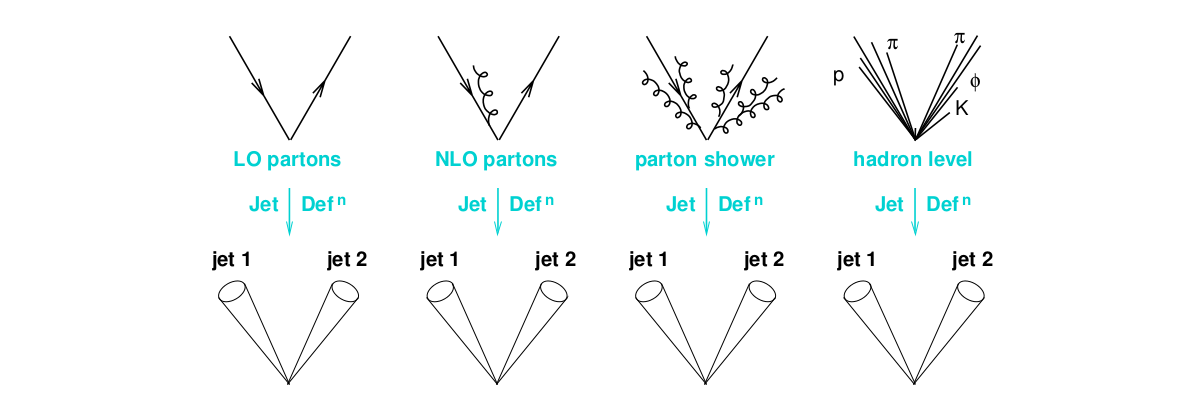
\includegraphics[width=1\textwidth]{Fig2/jetdefinition.png}
    \caption{The application of a jet definition to a variety of events that differ just through soft/collinear branching and hadronization should give identical jets in all cases~\cite{GavinLectures}.}
    \label{fig:jetdefinition}
  \end{center}
\end{figure}

Tradiontally, jet algorithms have been classified into two categories: cone algorithms and sequential recombination algorithms. 

Cone-like algorithms are based on the collinear nature of gluon radiation and the parton shower described above. The decay products of and emission from a hard quark or gluon will tend to form a cone of particles in the $\eta - \phi$ plane as they propagate.
% Then a cone of a suitable radius will capture these decay procuts.
An cone algorithm will work as follows~\footnote{This is how CMS cone algorithm, used for the preparation for the LHC running, works.}: first, it sorts all particles in the event according to their momentum, and identifies the one with largest $\pt$. This is referred to as seed particle. Then a cone of radius $R$ in  $\eta - \phi$ is drawn around the seed. The direction of the sum of the momenta of those particles is identified and if it doesn't coincide with the seed direction then the sum is used as a new seed direction, and iterates until the sum of the cone contents coincides withthe previus seed (this type of algorithm is cone ``iterative'' cone since it iterates the cone direction). This is how a stable cone is reached. A difficulty and major drawback in this procedure is the use of the transverse momentum of the particle to select the first seed. This definition is collinear unsafe, i.e. a splitting of the hardest particle into a nearly collinear pair can have the consequence that another, less hard particle, pointing in a different direction suddenly becomes the hardest in the event, leading to a different final set of jets. There are many other variants of cone algorithms, and nearly all suffer from problems of either collinear safety, or infrared safety (an extra soft particle creates a new seed, which can lead to an extra stable cone being found). A fix for these problems came in a algorithm called Seedless Infrared Safe Cone (SISCOne)~\cite{SISCone}.


Recombination algorithms, on the other hand, are both collinear and infrared safe. And for this reason, they can be used in calculations to any order in perturbation theory. The term recombination is used given that these algorithms work as if they were inverting the sequence of splittings of the parton shower. In general, recombination algorithms operate by successively combining pairs of particles using a distance metric, $d_{ij}$.  At hadron colliders, due to the fact that one of the incoming partons may continue along the beam, for every pair of particles this metric is compared to a so-called ``beam distance'', $d_{iB}$, and only when  $d_{ij}<d_{iB}$ the particle pair is combined and considered for subsequent clustering steps. 

ATLAS (and also CMS) has chosen anti-$k_t$~\cite{antiktalg} algorithm as the default jet algorithm for use in physics analysis.  This recombination algorithm as well as the Cambridge-Achen algorithm~\cite{CamAchen}, or C$/$A are extensions of the original $k_t$ algorithm developed for the analysis of multi-jet events at $e^+ e^-$ colliders~\cite{JADE} and subsequently extended for use at hadron colliders~\cite{kt2}~\cite{kt1}. In this thesis, the $k_t$ algorithm was used for jet substructure studies, see section~\ref{sec:substructure}.

The orginal $k_t$ algorithm implements the following (\ref{eqn:origkt}) distance metric between particles $i$ and $j$,

\begin{equation} 
d_{ij} = \frac{2E_i E_j (1-cos\theta_{ij}) }{Q^2}
\label{eqn:origkt}
\end{equation}

where $Q$ is the total energy in the event, $E_i$ is the energy of particle $i$ and $\theta_{ij}$ the angle between particles $i$ and $j$. In the collinear limit, $d_{ij}$ is related to the relative transverse momentum between particles $i$ and $j$ (hence the name $k_t$ algorithm), normalized to the total visible energy.
The particles are combined if the minimum $d_{ij}$, $d_min$, is below a certain threshold, $y_{cut}$.  The jet multiplicity depends on the value of $y_{cut}$, as a lower value will result in more soft or colliinear emissions surviving as jets. %This is thus the first definition of an ``event shape'', this threshold marks the transition between two-jet events and three-jet events.
As mentioned above, for hadron colliders, the notion of a beam distance is added. A distance scale, $\Delta R = \sqrt{\Delta y^2 +\Delta \phi^2}$, is introduced to define the typical radius for a jet, effectively replacing $y_{cut}$. In this case for every pair of particles a new distance is define, (\ref{eqn:kt}),

\begin{equation} 
d_{ij} = min(p^2_{ti},p^2_{tj}) \frac{\Delta R^2_{ij}}{R^2}
\label{eqn:kt}
\end{equation}

and the beam distance, $d_{iB}=p^2_{ti}$. %, in the way that when no particle j is found such that $\Delta R_{ij} < R$ then i is promoted to the status of a jet. 
The algorithm proceeds by searaching for the smallest of the $d_{ij}$ and the $d_{iB}$. If it is a $d_{ij}$ then particles $i$ and $j$ are recombined into a single new particles. If it is a $d_{iB}$ then $i$ is removed from the list of particles, and called a jet. This is repeated until no particles remain.

As opposed to cone algorithms, for the $k_t$ algorithm, the jets have quite irregular shapes, and particles with $\Delta R_{ij} > R$ can still be clustered within the jet. This is a problem when, for example, an irregularly shaped jet happens to extend into poorly instrumented detector regions. Another drawback of this definition is that soft particles are clustered first. This  has the potential to introduce complications when the detector noise of energy density fluctuations are large.

A feature of the $k_t$ algorithm that is attractive is that it not produces jets but also assigns a clustering sequence to the particles within the jet. It is possible then to undo the clustering and look inside the structure of the jet. This has been exploited in a range of QCD studies, and also in searches of hadronic decays of boosted massive particles  and will be used here for the search of two-pronged jets in gluon splitting.

The prescription above may be generalized beyond the $k_t$ algorithm. By inverting the power law in the particle distance metric, $d_{ij}$, the anti-$k_t$ algorithm is obtained. The particle distance metric used by this algorithm is,

\begin{equation} 
d_{ij} = min(p^{-2}_{ti},p^{-2}_{tj}) \frac{\Delta R^2_{ij}}{R^2}
\label{eqn:antikt}
\end{equation}

and the  beam distance, $d_{iB}=p^{-2}_{ti}$. This definition results in the clustering of the hardest emissions first. This has several benefits in the context of high-luminosity hadron collisions.

Note that the anti-$k_t$ algorithm does not provide useful information on jet substructure if a jet contains two hard cores, then the $k_t$ (or C/A) algorithms first reconstruct those hard cores and merge the resulting two subjets. The anti-$k_t$ will often first cluster the harder of the two cores and then gradually aglomerate the contents of the second hard core.

These algorithms, and more, are implemented in {\sc Fastjet}~\cite{fastjet} software package for jet-finding. 


%------------------------------------------------------------------------
\subsection{Jet substructure}\label{sec:substructure}
%------------------------------------------------------------------------

The study of a quantity related to the distributions and multiplicity of particles in the event phase space lead to the first evidence of jet structure, as pointed out in ref.~\cite{PhysRevLett.35.1609}. In general, all final hadronic states in $pp/p\bar{p}/e^+e^-$ collisions can be explored in terms of the structure and shape of the event energy flow by means of so called ``event shape'' variables. This family of variables attempt to extract information about the global geometry of an event, usually distinguishing between di-jet events and multijet final states. Such variables have been successfully utilized in many SM measurements and BSM searches, see for example~\cite{Abbiendi:2007aa}\cite{Aad:2012np}. 

Although very useful, event shape variables are not sensitive to the detailed structure and distribution of energy inside a particular jet in the event. In new physics searches, tools for the identification of individual objects that might be signature of new particles are desired. For example, when an unstable particle with large transverse momentum decays hadronically, the final state may contain a number of nearly collinear jets. These jets may be merged by a jet finder; %The decay products of boosted heavy quarks or bosons might be reconstructed as a single jet, 
a method for selecting these jets would allow for the study of their properties.
  This interest lead to the development of a wide range of jet substructure techniques in the recent years.

  Jet substructure methods probe the internal structure of jets from a detailed study of its constituents (see chapter\ref{sec:reconstruction}). These techniques have been first thought for distinguishing boosted hadronic objects from the background of jets initiated by light quarks and gluon, see for example~\cite{ATLASBoostedHbb},
%http://cdsweb.cern.ch/record/1201444/
but they have been also used succesfully in other applications, including separating quark jets from gluon jets~\cite{PhysRevLett.107.172001} and identifying boosted decay producs in new physics~\cite{PhysRevD.82.095012}.

%Jet shapes and jet algorithms in SCET, by Ellis, Vermillon, et all
Jet shapes, which are event shape-like observables applied to single jets, are an effective tool to measure the structure of individual jets~\cite{springerlink:10.1007/JHEP11(2010)101}.% {\bm ELEGIR REFERENCIA}. 
 The shape of a jet no only depends on the type of parton (quark or gluon) but is also sensitive to non-perturbative fragmentation effects and underlying event contributions~\cite{ATLASJetShapes}.


%from Jet substructure at the Tevatron and LHC
%Observables desinged to be sensitive to the internal structure of jets are expected to also be sensitive to pile-up. Large-radius jets, such as those used in the measurements of jet substructure, are naturally more susceptile to pile-up due to their larger catchment area~\cite{CatchmentArea}; the invariant mass of these large jets is particularly affected. %http://arxiv.org/abs/1009.1143
%Techniques for correcting these effects or mitigating their impact $-$such as the splitting and filtering procedure pioneered in ATLAS$-$  are essential in producing precision measurements for several of the analyses presented by the Tevatron and LHC experiments.  A more thorough review of these issues at ATLAS can be found in~\cite{DavidMillerThesis}


In the particular case of the present analysis, several distinguishing characteristics between jets originating from $b$-quarks and jets originating from the the splitting of a gluon into a $b\bar{b}$ pair can be determined using the techniques of jet substructure. 


\subsubsection{Jet width}


%From http://www.springerlink.com/content/54748j617818718q/?MUD=MP
The jet width is part of a set of continuous variables that try to distinguish individual particles/subjets within the jet as a smooth funcion of $(\delta \eta, \delta \phi)$ away from the jet axis, in order to form combinations like geometric moments.  This particular combination sums the distances between the jet constituents and its axes, weighted by the constituent $\pt$, and then normalized to the total $\pt$ of the jet. The compact definition is 

%\begin{equation} 
%g = \sum_{i\in jet} \frac{p^i_T}{p^{jet}_T} |\Delta R_i|
%\label{eqn:girth}
%\end{equation}
%where $\Delta R_i = \sqrt{\Delta y^2_i + \Delta \phi^2_i}$

\begin{equation} 
\mbox{ {\it Jet width}} = \frac{\sum_{i=1}^N \pt^{const_i} \,\Delta R (const_i,jet) }{\sum_{i=1}^N \pt^{const_i} }
\label{eqn:trackjetwidth}
\end{equation} 
where $N$ is the total number of calorimeter or track constituents.  This observable is also highly correlated to the mass of the jet.

This linear radial moment is a measure of the width or ``girth''~\cite{PhysRevLett.105.022001} of the jet.  Under the assumption of central jets with massless constituents at small angles, this linear moment is identical to jet broadening~\cite{Catani1992269}, defined as the sum of momenta transverse to the jet axis normalized by the sum of momenta. While jet broadening is natural at an $e^+ e^-$ collider, the linear radial moment is more natural at the LHC.

An alternative approach to measuring the width is to use the angular separation of the two hardest constituents inside jets. This has the advantage of effectively removing any dependence on the shower development within the calorimeter and focuses on the hard component of the jet.



%Measurement of QCD jet broadening~\cite{PhysRevD.44.601}.In this paper, we discuss the use of an event-shape parameter QT introduced by Ellis and Webber to describe hadronic final states in proton-antiproton collisions [18]. QT is defined as the scalar sum of the momenta perpendicular to the transverse thrust axis, where the transverse thrust axis represents the direction of maximum energy flow in the plane transverse to the beam. It has the property of being both finite and calculable for all multiparton final-state configurations, the case where particularly singularities occur in perturbation theory associated with the collinear emission of gluons. The behavior of QT with increasing energy is termed jet broadening because of its sensitivity to the increasing multiparton nature of a jet as the energy of the jet increases. % $Q_T / E_T$ ~ similar behavior with $E_T$ as Jet Width.

%Jet Angularities~\cite{springerlink:10.1007/JHEP11(2010)101} are also radial moments, but their “radial distances” are rescaled into the angular coordinates appropriate for $e^+ e^−$ event shapes. 



\subsubsection{Eccentricity}

In defining a jet moment there are several ways to weight the momentum and define the center of the jet. We have defined the jet width as the first moment of the transverse energy with respect to the jet axis; another example of useful combination is the jet pull~\cite{PhysRevLett.105.022001}. But it is also natural to look at higher moments, such as those contained in the covariance tensor,

\[ C = \sum_{i\in jet}\frac{p^i_T|r_i|}{p^{jet}_T} \left( \begin{array}{cc}
 \Delta y^2_i & \Delta y_i \Delta\phi_i \\ 
 \Delta\phi_i \Deltay_i & \Delta \phi^2_i \end{array} \right). \]


Here, $\vect{r}_i = (\Delta y_i, \Delta \phi_i) = \vect{c}_i - \vect{J}$, where $\vect{J} = (y_J,\phi_J)$ is the location of the jet and $\vect{c}_i$ is the position of a cell or particle with transverse momentum $p^i_T$. The eigenvalues $a \geq b$ of this tensor are similar to the semimajor and semiminor axes of an elliptical jet. The jet eccentricity, defined below, is a combination of these eigenvalues, and it is a measure of how elongated is the area of a jet.

\begin{equation} 
e = \sqrt{\frac{(a^2 - b^2)}{a}}
\label{eqn:ecc}
\end{equation}

%No significan difference in eccentricity was found between quark and gluon jets.


\subsubsection{Jet Mass}


The jet mass, like the linear radial moment, also depends on the radiation pattern of the event. It is the most basic observable for disinguishing massive boosted objects from jets originating from quarks or gluons. The latter are expected to be dominated by wide-angle emissions, with increase probability to see high mass jets initiated from gluons as opposed to quarks~\cite{PhysRevD.79.074012}.  


{\sc Need to complete this}.


%In the recent ATLAS analysis of 35~pb$^{-1}$ of data, the sensitivity of individual jet mass to pile-up is directly tested (for jets with at least 300~GeV). The mean jet mass is observed to increase linearly with NPV~\cite{ATLAS-CONF-2011-073}. %The filtering procedure significantly reduces the effect of pile-up on jet mass.




\subsubsection{Subjet multiplicity}

With the development of the $k_t$ algorithm, subjets were first used in the description of the hadronic final state in $e^+e^-$ annihilation, such as the study of the jet multiplicity at different energy scales~\cite{Catani1992445}. By using the sequential recombination algorithms introduced in the previus section, it is straightforward to define a ``subjet algorithm'' in which the structure of the jet's constituents is resolved using either the same jet finder algorithm or a new one with a fixed (smaller) distance parameter.

The subjet multiplicity $-$ the number of subjets within a jet $-$ provides information on the distribution of energy and multiplicity of particles within a jet. For instance, in~\cite{Snihur1999494} the result of meassuring this ``radiation variable'' on quark- and gluon-initiated jets indicates that gluon-initiated jets tend to have on average higher subjet multiplicity. This result is consistent with the QCD prediction that gluons radiate more than quarks. In the case of this and different other analyses % see for instance  http://iopscience.iop.org/1126-6708/1999/09/009/
the $k_t$ algorithm is rerun for subjet finding.

As an alternative to fixed distance parameter subjets, it is also possible to undo the last step in the recombination sequence~\cite{kt2} in order to identify the decay products of an object.  This approach is used in seveal jet grooming procedures\footnote{Jet grooming comprises dedicated techniques to remove uncorrelated radiation within a jet. A review of these procedures can be found in~\cite{Abdesselam:2010pt}. }, see for instance~\cite{pruning}.

%In contrast to the $k_t$ algorithm, it is not useful just to undo the last stage of C/A clustering: The absence of any momentum scale in its distance measure means that the last clustering often involves soft radiation on the edges of the jet and so, is unrelated to the heavy object's decay. 
%The so-called BDRS method of jet grooming
%http://prl.aps.org/abstract/PRL/v100/i24/e242001
% uses the C/A algorithm. Subjets are then defined by de-clustering the C/A algorithm and evaluating the relative mass of the subjets compared to the parent jet. As a final step, the three hardest identified subjets are recombined to define the resulting ``filtered'' jet.

It is also possible to extend the use of individual subjets in conjunction with more traditional jet shape variables. Using these tools, an inclusive jet shape based on the substructure topology of a single jet, ``$N$-subjettiness''~\cite{nsubjettiness} is defined.





\subsubsection{$N$-subjettiness}

As mentioned above, the $N$-subjettiness~\cite{nsubjettiness} is a jet shape that describes the energy flow within a jet. It quantifies the degree to which  radiation is aligned along specified subjet axes. This jet shape was adapted from the event shape $N$-jettiness~\cite{njetti}.

Given candidate subjets directions determined by an external algorithm such as the exclusive $k_t$ procedure~\cite{exclusivekt}, the variables is defined as,


\begin{equation} 
\tau^{(\beta)}_N = \frac{1}{\sum_k {\pt}_k\,(R_0)^{\beta}} \sum_k {\pt}_k (\min \{ \Delta R_{j1,k},\,\Delta R_{j2,k},...,\,\Delta R_{jN,k} \})^{\beta}
\label{eqn:nsubjet}
\end{equation} 

The sum runs over the $k$ constituent particles in a given jet where $p_{T,k}$ are their transverse momenta, and $\Delta R_{j1,k}$ is the distance between the candidate subjet $j1$ and a constituent particle $k$.  $R_0$ is the characteristic jet radius used in the original jet clustering algorithm.
The exponential weight, $\beta$, can optionally be applied to the angular distance computed between the subjets and the jet constituents.  

This jet shape was designed to identify boosted $N$-prong hadronic decays. With $\beta=1$, the definition above indicates that jets with $\tau_N\approx 0$ have all their radiation aligned with the candidate subjet directions and therefore have $N$ (or fewer) subjets. Jets with $\tau_N\gg 0$ have a large fraction of their energy distributed away from the candidate subjet direction and therefore have at least $N+1$ subjets.

To separate boosted hadronic objects from the QCD jet background, one could use the complete set of  $\tau_N$ (with different values of $\beta$) in a multivariate analysis. However, \cite{nsubjettiness} showed that a simple cut on the ratio $\tau_N/\tau_{N-1}$ provides excellent discrimination power for $N$-prong hadronic objects. In particular, $\tau_2/\tau_1$ can identify boosted $W/Z$ and Higgs bosons, with the angular weighting exponent $\beta =1$ providing the best discrimination.

Since eq.~\ref{eqn:nsubjet} is linear in each of the constituent particle momenta, this variable is an infrared- and colliner-safe observable.  In subsequent work~\cite{mininsubjettiness}, Thaler and van Tilburg showed that the initial step of choosing candidate subjet axes is in fact unnecessary. In particular, the quantity in equation~\ref{eqn:nsubjet} can be minimised over the candidate subjet directions, further improving boosted object discrimination.

The definition of $N$-subjettiness is not unique, and different choises can be sued to give different weights to the emissions within a jet. There generalizations of $N$-subjettiness are similar to different ``angularities''~\cite{angularities} used in $e^+e^- \rightarrow$hadrons measurements.


%From Nsubjettiness paper
%use $N$-subjettiness to effectively ``count'' the number of subjets in a jet. Compare to previous jet substructure techniques, $N$-subjettiness  has the advantage of finding jets that contain two or more lobes of energy.
%Subjet candidates where determined by using the exclusive $k_t$ algorithm, forcing it to return exactly $N$ jets.


